\section{Anvendt rotårsaksanalyse}
Metoden innebærer syv steg (visualisert i figur \ref{fig:prosess}), der hvert steg anbefaler et sett verktøy for å fullføre det. Bruk av et eller flere verktøy kommer helt an på problemet som skal løses. Valg av verktøy i hver fase er i stor grad basert på flytdiagrammene i boken av Andersen og Fagerhaug \cite{RCA}, som beskriver hvordan en velger riktig verktøy i hvert steg, for et bestemt problem. Selv om verktøyvalg er godt beskrevet tok vi med vår egen vurdering på hvilke verktøy som skulle brukes, siden boken ikke er direkte tilpasset informasjonssikkerhetsoppgaver. Vi har også brukt noen få verktøy utover det boken anbefaler når det kommer til dataanalyse. 

\begin{figure}[H]
    \centering
    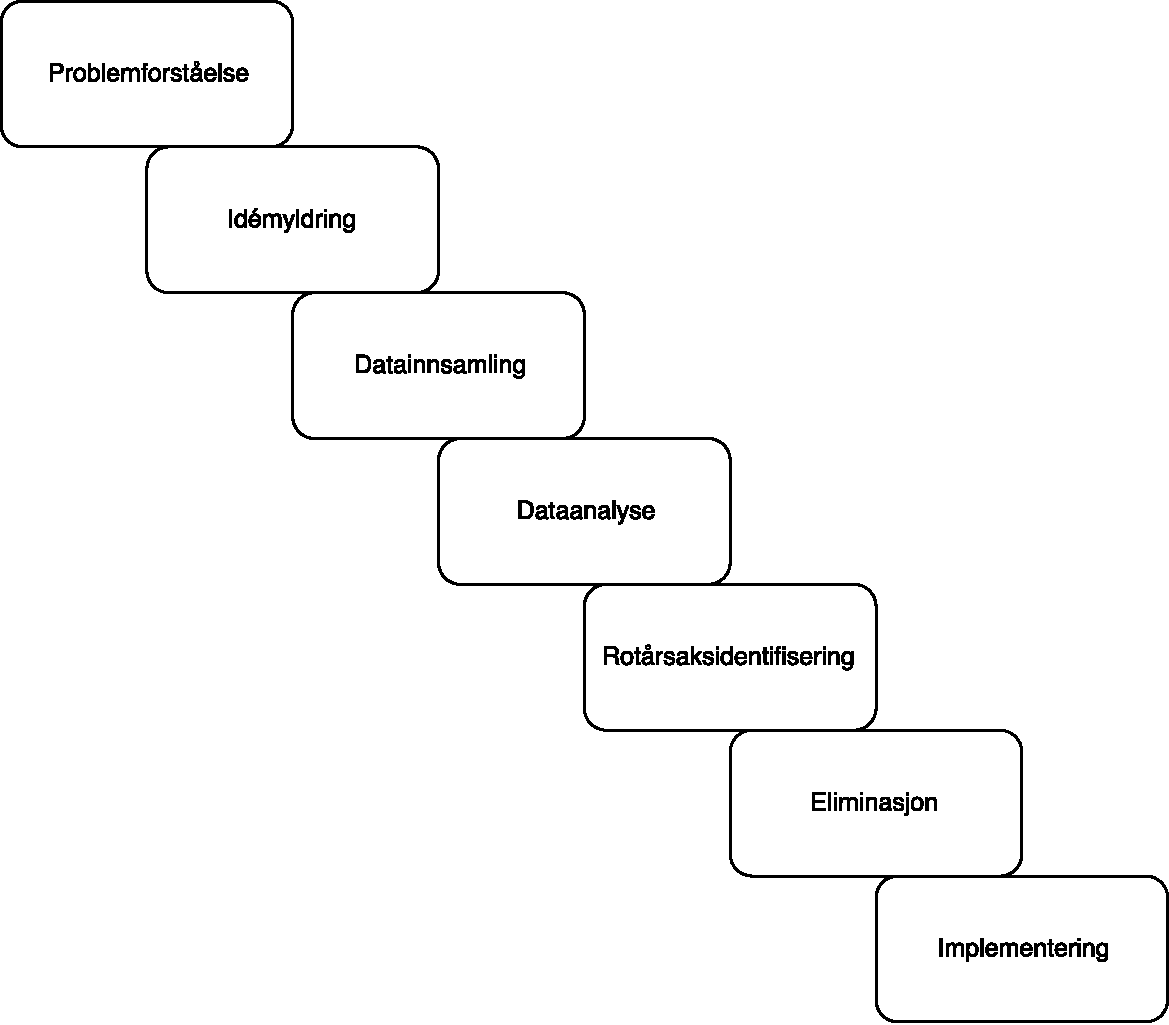
\includegraphics[scale=0.6]{prosess}
    \caption[RCA-prosess]{De syv fasene i rotårsaksanalyseprosessen}
    \label{fig:prosess}
\end{figure}

\subsection{Problemforståelse}
Problemforståelse går ut på å få en solid forståelse for problemet en ønsker å løse og kan også hjelpe med å skape enighet rundt hva problemet egentlig omfatter. Det er også viktig for å passe på at ressursene som benyttes i analysen brukes effektivt videre. Under beskrives de verktøyene som ble brukt av oss i denne fasen. 

\subsubsection{Flytdiagram}
Et flytdiagram viser flyten av aktiviteter i en prosess. I informasjonssikkerhet kan det brukes som en metode for å konkretisere og illustrere et problem ved eller angrep mot virksomhetens aktiva. Formålet er å skape en detaljert forståelse for en prosess som har noe med problemet å gjøre \cite{RCA}.

\subsubsection{Kritiske hendelser}
Hovedpoenget med kritiske hendelser er å identifisere de mest kritiske symptomene i problemet. Det kan hjelpe med å forstå hvilke aspekter ved problemet som trenger å løses, samt forstå problemets natur og konsekvenser for virksomheten \cite{RCA}. Innen informasjonssikkerhet har man ofte logger med hendelsesdata. Det gjør det naturlig å bruke kritiske hendelser siden informasjonen ofte eksisterer på forhånd og trenger bare å bearbeides. 

\subsubsection{Ytelsesmatrise}
Ytelsesmatrise er et diagram som tar i betraktning viktigheten og den nåværende ytelsen til en variabel. Dette gjør at man enkelt kan vurdere hvilken prioritering variablene som blir analysert har \cite{RCA}. Matrisen går fra en til ni på hver akse og er delt inn i fire like store hjørneområder. Ut i fra hvor høy ytelse ytelse og hvor viktige de er, er variablene enten: uviktig, overdrevent, må forbedres eller ok. I informasjonssikkerhet kan det brukes til å vurdere virksomhetens aktiva opp mot for eksempel eksisterende kontroller.

\subsection{Idémyldring}
Målet med idémyldring er å generere så mange idéer som mulig om et gitt emne. I rotårsaksanalyse er målet stort sett å generere en liste over problemområder som kan forbedres, identifisere mulige konsekvenser, generere en liste over mulige årsaker til problemet og oppmuntre til å tenke på løsninger som kan eliminere problemet. Det finnes i hovedsak to typer idémyldring: strukturert og ustrukturert. I strukturert idémyldring har hver deltaker sin tur til å komme med idéer. Dette fører til lik deltagelse og at ingen dominerer prosessen med egne idéer. I ustrukturert idémyldring kan hvem som helst komme med idéer når som helst. Dette er ofte mer spontant, men kan føre til at en person dominerer prosessen \cite{RCA}. 

\subsubsection{Nominell gruppeteknikk (NGT)}
Nominell gruppeteknikk er en strukturert metode for idémyldring som hjelper med å gå fra mange idéer, til å sitte igjen med de beste. Konseptet går ut på å myldre idéer og skrive dem ned på lapper, for så å anonymt gi idéene poeng fra en til fem. Et tallpoeng kan bare gis én gang. Til slutt blir tallene lagt sammen og du sitter igjen med de beste idéene. 

\subsection{Datainnsamling}
Ustrukturert og tilfeldig problemløsning har en tendens til å bli svært unøyaktig. Strukturert rotårsaksanalyse gir derimot et godt grunnlag for blant annet datainnsamlingen, som er en av de sentrale fasene i prosessen. Under beskrives verktøyene som ble brukt for å samle inn informasjon. 

\subsubsection{Spørreundersøkelser}
Spørreundersøkelser brukes når en er på utkikk etter å samle inn data om personers holdninger, følelser eller meninger om et spesifikt problem. En kan skille mellom to typer spørreundersøkelser: kvalitative og kvantitative spørreundersøkelser. Kvantitative undersøkelser handler om å få mange svar slik at en kan ta avgjørelser basert på tall som kan brukes til statistisk analyse. Kvalitative undersøkelser går ut på å samle detaljert informasjon om emnet. Dette kan hjelpe med blant annet å formulere hypoteser for å dirigere kvantitativ undersøkelse senere, eller å komplimentere en kvantitativ undersøkelse ved å bruke sitater fra åpne spørsmål \cite{KvalKvant}. Det brukes ofte elementer fra begge typene når en spørreundersøkelse lages. Når det er snakk om informasjonssikkerhet kan kvalitative undersøkelser brukes når det for eksempel skal samles inn informasjon om brukervaner på nett, eller grad av kunnskap og erfaring om informasjonssikkerhet. Kvalitative undersøkelser kan brukes når det kreves detaljert informasjon om et system eller indre forretningsprosesser. 

\subsubsection{Sampling}
Hovedpoenget med sampling er å trekke ut deler av en populasjon, for å trekke konklusjoner om denne uten å trenge å undersøke alle enhetene \cite{wiki:sample}. I rotårsaksanalyse kan det brukes for å effektivt samle inn data om problemer eller årsaker, og skaffe en bedre forståelse av situasjonen \cite{RCA}.

\subsection{Dataanalyse}
I denne fasen blir dataene analysert og visualisert. Hovedmålet er å avklare mulige rotårsaker som har innvirkning på problemet, og hvilke av de som har størst innflytelse. Under beskrives de ulike verktøyene som ble brukt for å analysere dataene.

\subsubsection{Histogram}
Histogrammer, også kjent som søylediagram, brukes for å vise distribusjon og varians i et datasett. Dataene kan vises i form av lengde, tid, kostnad, mengde osv. Hovedoppgaven til et histogram er å presentere data på en oversiktlig måte slik at det er lett å se mulige relasjoner. I rotårsaksanalyse brukes det til å se hvilke årsaker som dominerer og for å forstå distribusjonen av forskjellige problemer, årsaker, konsekvenser osv. \cite{RCA} Det er viktig å ha minst 30 svar for å lage et gyldig histogram \cite{RCA}.

\subsubsection{Affinitetsdiagram}
Affinitetsdiagram er et verktøy som kan brukes til å analysere kvantitative data. Formålet er å gruppere svar for å finne underliggende relasjoner mellom de resterende gruppene \cite{RCA}. I vår rotårsaksanalyse ble det brukt til å utforske relasjoner mellom forskjellige årsaker, og gruppere relaterte årsaker inn i klasser som kan analyseres kollektivt senere. 

\subsubsection{One-way ANOVA}
ANOVA, også kjent som variansanalyse, er en samlebetegnelse på en rekke statistiske metoder som tester likhet mellom to eller flere utvalg, der én eller flere faktorer gjør seg gjeldene \cite{ANOVA}. 

\subsubsection{Independent-samples t-test}
Dette er en type t-test som brukes for å teste gjennomsnittet mellom to uavhengige grupper på samme avhengige variabel \cite{t-test}. 

\subsection{Rotårsaksidentifisering}
De foregående fasene skal ha generert en liste over mulige rotårsaker og målet i denne er å identifisere de faktiske årsakene. Det kan kreves flere iterasjoner for å finne rotårsaken(e). Verktøy som ble brukt til identifisering er beskrevet under. 

\subsubsection{Årsak-virkningsdiagram (Fiskebeindiagram)}
Et typisk årsak-virkningsdiagram undersøker og analyserer relasjonen mellom et problem og dets årsaker. Det fungerer som en kombinasjon av idémyldring og systematisk analyse. Det brukes for å generere og gruppere årsaker, og evaluere årsakene til problemet for å finne ut hvilke som mest sannsynlig er rotårsaker. Det finnes to typer årsaks-virkningsdiagrammer: fiskebeindiagram og prosessdiagram. Et prosessdiagram er egentlig en samling av fiskebeindiagrammer der hver prosess har sitt eget diagram. Det finnes to ulike tilnærminger til å skape et fiskebeindiagram: spredningsanalyse og årsaksopplisting. Kort forklart, spredningsanalyse grupperer først og idémyldrer etterpå, mens årsaksopplisting idémyldrer først og grupperer etterpå \cite{RCA}. 

\subsubsection{5 Whys}
5 Whys brukes for å undersøke høyere nivåer av årsaker. Som navnet beskriver, går det ut på å spørre ``Why?'' til en bestemt årsak for å komme frem til en ny årsak. Deretter blir det stilt spørsmål til den nye årsaken. Dette gjentar seg helt til det ikke er noen relevante årsaker å komme med. Den siste er da rotårsaken. Som en tommelfingerregel itererer man gjerne fem ganger, men det kan være både flere og færre avhengig av tilfellet. 

\subsubsection{Feiltreanalyse}
Feiltreanalyse er en top-down, deduktiv analyse der en uønsket tilstand av et system analyseres ved hjelp av boolsk logikk for å kombinere en rekke hendelser \cite{wiki:faulttree}. I RCA brukes det for å få en klar oversikt over mulige årsaker, og for å se relasjoner mellom årsaker eller identifisere grupper med relaterte årsaker \cite{RCA}. 

\subsection{Problemeliminering}
Denne fasen innebærer å komme med mulige løsninger til problemet for å eliminere rotårsaken. Boken til Fagerhaug og Andersen \cite{RCA} beskriver to mulige tilnærminger til denne fasen. En tilnærming for å stimulere kreativitet når man leter etter løsninger, og en for å konstruere og utvikle løsninger. Vi har prøvd et verktøy fra hver tilnærming og de er beskrevet under. 

\subsubsection{De seks tenkehattene}
Formålet med de seks tenkehattene er å oppmuntre til å se problemet og løsningene fra forskjellige synsvinkler. Konseptet går ut på at personene får hver sin hatt som skal illustrere deres holdning til problemene \cite{RCA}. 

\begin{description}
    \item[Hvit hatt] skal være kald, nøytral og objektiv, personen skal fokusere på fakta.
    \item[Rød hatt] skal representere sinne, og skal bare fokusere på magefølelsen og egne følelser.
    \item[Svart hatt] skal være pessimistisk og negativ, og fokusere på hvorfor idéen er dårlig.
    \item[Gul hatt] er optimistisk og positiv, og skal fokusere på hvorfor idéen er bra og vil fungere.
    \item[Grønn hatt] representerer gresset, fruktbarhet og vekst, og skal fokusere på å vøre kreativ og komme på nye idéer.
    \item[Blå hatt] er koblet til himmelen, og skal fokusere på å se tingene fra et høyere perspektiv.
\end{description}

\subsubsection{Systematisk Innovativ Tenkning (SIT)}
SIT er en problemelimineringsmetode som baserer seg på konseptet om en ``lukket verden''. Dette betyr at den fokuserer på at løsningene på problemet ofte finnes i det fagområdet problemet eksisterer i. SIT baserer seg på å undersøke en eller flere kjernekomponenter ved hjelp av fem hovedprinsipper \cite{RCA}: 

\begin{description}
    \item[Attributtavhengighet] vurderer å endre en nøkkelvariabel i et produkt for å skape forbedring.
    \item[Komponentkontroll] ser på hvordan et produkt er knyttet til omgivelsene.
    \item[Erstatning] handler om å erstatte en del av et produkt med noe annet fra produktets omgivelser.
    \item[Forkastning] vurderer å forbedre problemet ved å fjerne en komponent. 
    \item[Oppdeling] har som mål å splitte et produkts attributter i to, som for eksempel splittelsen av sjampo fra balsam.
\end{description}

Hovedprinsippet i vårt prosjekt er å fokusere på at løsningene er tilknyttet fagområdet informasjonssikkerhet.

\subsection{Løsningsimplementering}
I den siste fasen er målet å implementere løsningene som ble funnet i foregående fase. I vår rapport vil implementeringen beskrives til beste evne, men ikke implementeres siden vi ikke har mulighet til dette. Implementeringen inkluderer blant annet organisering, utvikling av en implementeringsplan, skape et konsensus om de nødvendige endringene og selvfølgelig implementeringen. Implementeringen av løsningen kan sies å være en suksess når symptomene forsvinner. Verktøyene beskrives under.

\subsubsection{Trediagram}
Et trediagram er et verktøy som er enkelt å bruke og er passende for å dele opp større oppgaver inn i mindre, mer håndterlige aktiviteter. Det er et verktøy som hjelper til å organisere arbeidet som må gjennomføres for å implementere tiltakene som er anbefalt. I informasjonssikkerhet kan dette benyttes for å strukturere oppgavene og planlegge implementeringsprosessen av løsningen. Et trediagram visualiserer hierarkiet i aktivitetene som må gjennomføres, eller enklere sagt, rekkefølgen av gjøremål for å fullføre implementeringen. 

\subsubsection{Kraftfeltsanalyse}
En kraftfeltsanalyse er basert på den oppfatningen at alle situasjoner er resultatet av krefter som virker for og i mot den faktiske tilstanden. En forandring i disse kreftene vil fremkalle en endring, noe som kan brukes til å endre ting i ønsket retning. I rotårsaksanalyse brukes det for å få innsikt i endringsklimaet til en mulig implementering, samt å planlegge aktiviteter som skal til for å implementere løsningen \cite{RCA}. Verktøyet kartlegger krefter som virker for endringen, og krefter som virker i mot. 